\chapter{La mise en place d’Archifiltre dans la chaîne en pré-traitement \protect\footnotemark}
\footnotetext{Entretien avec Chloé Moser (18 avril 2024)}


Une chaîne de traitement se dessine donc au fur et à mesure des années et particulièrement des différents développements du Programme \gls{VITAM}. Un modèle émerge pour la gestion des archives électroniques à l’échelle des Ministères, le versement dans le \gls{SAE} \gls{VITAM} et pour ce faire le traitement des archives via le logiciel ReSIP en amont. Au sein du service des archives des Ministères sociaux, à l’époque Ministère des solidarités, de la santé, du travail et de la Jeunesse et des Sports, on se rend compte en parallèle du besoin d’un outil de pré-versement notamment pour aider les archivistes à gérer les vracs, constituant alors 80 \% des archives numériques, et les comprendre alors que l’outil informatique les rend plus difficile à appréhender que ce que le métier connaît face aux archives papiers.

\subsection{Genèse d’Archifiltre}
Le projet \gls{Archifiltre},  initié en 2016, est né au sein des Ministères sociaux . Ce sont les premières expériences de traitement d'archives numériques et notamment celui effectué par Marie Jenner, stagiaire TNAH aux Ministères sociaux, sur un vrac numérique, qui démontrent la différence fondamentale entre l’appréhension d’un fonds papier et d’un fonds numérique pour les archivistes. L’impossibilité de visualiser la totalité d’une arborescence et d’être réduit à se perdre dans des ouvertures de dossiers puis de sous-dossiers et ainsi de suite empêche le professionnel de l’information d’appréhender pleinement le fonds et de le traiter efficacement selon les méthodes connues. En deux mois, Marie Jenner avait réussi à traiter seulement 6 \% d'un versement de 6 Go. Le besoin de faire évoluer les pratiques pour s’adapter au support numérique et donc de créer des outils pour le faire s’impose alors déjà.


C’est l’archivage entraîné par le passage de la présidence de François Hollande à celle d’Emmanuel Macron en mai 2017 qui s’avère déterminant. Il met en exergue l’explosion de la production et donc de la  collecte d’archives numériques (1,7 To) faisant ainsi apparaître nettement  l'urgence de trouver des solutions pour traiter ces volumes avec des équipes dont le nombre n’augmentera pas. En effet, jusqu’alors les formations archivistiques en France mettaient l’accent sur le traitement et l’archivage de base de données. Or, la majorité des archives numériques à traiter s’avèrent être des documents bureautiques. Les professionnels se retrouvent donc démunis face à une telle masse de documents numériques à traiter\footcite[p.20]{scopsi_quels_2024}.
\begin{figure}[h]
	\centering
	\begin{minipage}[b]{0.45\textwidth} %Crée une sous-structure dans le document qui prend ici 45% de la largeur totale de la ligne.
		\centering
		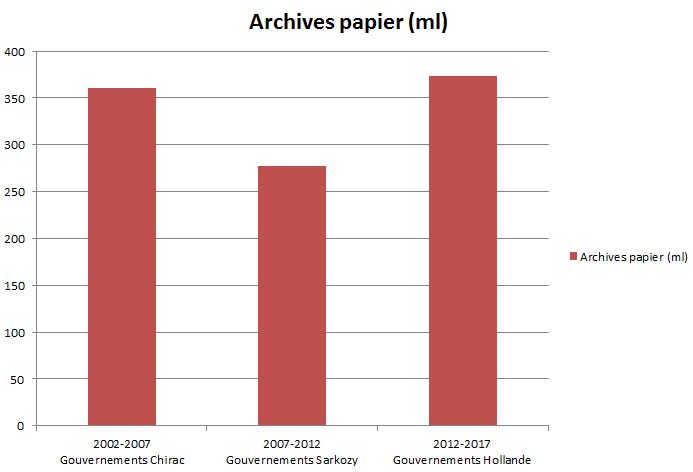
\includegraphics[width=\textwidth]{illustrations/figure7.1.png}
		\caption{Diagramme de l’évolution des volumes d’archives papiers collectés}
		\label{figure7.1}
	\end{minipage}
	\hfill %Met un espace entre les deux images.
	\begin{minipage}[b]{0.45\textwidth}
		\centering
		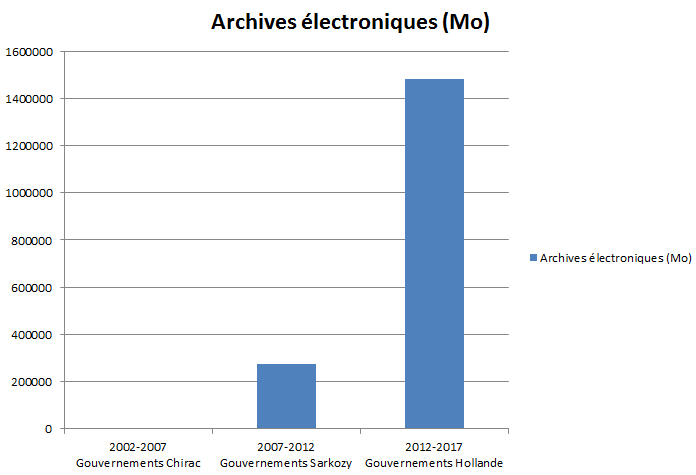
\includegraphics[width=\textwidth]{illustrations/figure7.2.png} 
		\caption{Diagramme de l’évolution des volumes d’archives  électroniques collectés}
		\label{figure7.2}
	\end{minipage}
	\caption{Comparaison de l'évolution des volumes d'archives papiers et électroniques collectés\protect\footnotemark}
	\label{fig:sidebyside1}
\end{figure}
\footnotetext{\textit{Présentation \gls{Archifiltre}}, modèle 2019}

Répondant au programme Entrepreneur d'Intérêt Général\footnote{\enquote{Les Entrepreneur(e)s d’intérêt général (co)pilotent le lancement et l'accélération de services numériques conçus selon l'approche beta.gouv.fr en soutien aux politiques publiques.} (\cite{noauthor_entrepreneur_nodate})} (EIG), le projet \gls{Archifiltre} est alors proposé par Patrice Loriot,  chef du pôle gestion des connaissances (bureau des archives et de la documentation), adjoint au sous-directeur des services généraux et de l'immobilier, et Anne Lambert, cheffe du bureau des archives des Ministères sociaux puis présenté par Anne Lambert et Chloé Moser, adjointe à la cheffe de bureau des archives. Leur candidature a été retenue notamment pour son potentiel de réutilisation dans les différentes administrations et parce qu’il était destiné à un réseau dynamique : celui particulièrement actif et collaboratif des archivistes. Le projet se monte alors d’abord grâce à la collaboration de deux entrepreneurs d’intérêt général recrutés pour lancer l’outil  et les archivistes du service, originellement spécialisés dans les archives papiers, par le biais de nombreux ateliers pour adapter les concepts de visualisation aux archives numériques. Ce travail fait émerger le but principal d’\gls{Archifiltre} : rendre à l’archiviste la sérénité du traitement papier en lui fournissant un outil lui permettant de visualiser et d’intellectualiser efficacement les arborescences.

\subsection{Mise en place d’Archifiltre et développements}
Les réflexions ont rapidement abouti à une première version disponible dès février 2018. Le but était de pouvoir recueillir au plus vite des retours utilisateurs sur l’outil et ainsi des perspectives d’amélioration. Dès cette première parution, la visualisation des arborescences, dite \enquote{visualisation en stalactites}, s’est imposée comme un élément clé de l’outil. Autour de celle-ci, de nombreuses nouvelles fonctionnalités ont été mises en place comme les zooms ou l'ajout de tags directement sur la visualisation de l’arborescence.


\insererImage{0.3}{illustrations/figure8.png}{Visualisation en stalactites de l'application Archifiltre}{figure8}


Le développement d’un export au format CSV compatible avec l’outil de préparation de \gls{SIP} ReSIP a permis à \gls{Archifiltre} de s’inscrire dans la chaîne de préparation des  versements dans des \gls{SAE} basés sur la solution \gls{VITAM}, en particulier celui des Archives nationales. Le 29 novembre 2018, le premier versement aux Archives nationales est d’ailleurs effectué par les Ministères sociaux ayant utilisé pour la première fois la chaîne de traitement qui allait devenir commune : l’étude de l’arborescence avec \gls{Archifiltre}, la préparation du \gls{SIP} avec ReSIP et le versement dans ADAMANT basé sur la solution \gls{VITAM}. 


Par ailleurs, la crise sanitaire de 2020 a joué un rôle important dans l'accélération de l'adoption d'\gls{Archifiltre}. En effet, son utilisation s’est accrue notamment car les archives papiers étant inaccessibles en télétravail, le traitement des archives numériques s’est développé. Pendant cette période de télétravail forcé, le choix a été fait de consacrer du temps à la formation et à la documentation sur l’outil, une documentation détaillée a été créée et de nombreuses formations ont été dispensées aux archivistes souhaitant profiter de ce temps forcé en télétravail pour se mettre à l’archivage électronique. L’outil étant en début de chaîne de traitement, il a par ailleurs constitué pour beaucoup un moyen de commencer à appréhender les archives numériques et la transition vers cette nouvelle part du métier d’archiviste. En conséquence de la crise sanitaire, une très nette réduction de la production papier a été observée, tandis que la production  électronique continue d’augmenter, profitant également au développement d’\gls{Archifiltre}.


En 2022, \gls{Archifiltre} élargit son champ d'action avec le projet Archifiltre-Mails, un outil de visualisation et de tri des messageries, financé par un appel à projet. Cet élargissement illustre l'impact significatif d'Archifiltre dans la gestion et l’adoption de méthodes pour le traitement des archives numériques en France. Ce projet devient prioritaire et le reste jusqu’en janvier 2024 où le choix est fait de le mettre en pause au profit de la première application d’\gls{Archifiltre}, renommée \enquote{Archifiltre-Docs\footnote{En juillet 2024, l’équipe a fait le choix de renommer Archifiltre-Docs en \gls{Archifiltre} par souci de clarté et pour s’adapter à l’usage.}}.


Enfin, \gls{Archifiltre}, grâce à sa relative simplicité et son utilité pour la compréhension d’arborescences, a vu son audience grandir au-delà des archivistes pour s’élargir à des agents de services numériques, aux services producteurs et finalement au grand public\footnote{Un schéma récapitulatif des étapes du développement d'Archifiltre est disponible en annexe \ref{annexe1}.}.